\documentclass{article}
\usepackage{xcolor}
\usepackage{titleps}
\usepackage[letterpaper, margin=0.95in]{geometry}
\usepackage{url}
\usepackage{amsmath}
\usepackage{amssymb}
\usepackage{wrapfig}
\usepackage{float}
\usepackage{mathtools}
\usepackage{enumitem}
\usepackage{tabu}
\usepackage{parskip}
\usepackage{natbib}
\usepackage{listings}
\usepackage{graphicx}

\usepackage[many]{tcolorbox}
% https://tex.stackexchange.com/a/569249
\setcounter{secnumdepth}{5}
\setcounter{tocdepth}{5}
\makeatletter
\newcommand\subsubsubsection{\@startsection{paragraph}{4}{\z@}{-2.5ex\@plus -1ex \@minus -.25ex}{1.25ex \@plus .25ex}{\normalfont\normalsize\bfseries}}
\newcommand\subsubsubsubsection{\@startsection{subparagraph}{5}{\z@}{-2.5ex\@plus -1ex \@minus -.25ex}{1.25ex \@plus .25ex}{\normalfont\normalsize\bfseries}}
\makeatother

\usepackage{hyperref}
\usepackage[color=red]{todonotes}
\usepackage{forest}
\definecolor{light-yellow}{HTML}{FFE5CC}

\newpagestyle{ruled}
{\sethead{CMU 16-831}{Introduction to Robot Learning }{Fall 2026}\headrule
  \setfoot{}{}{}}
\pagestyle{ruled}

\renewcommand\makeheadrule{\color{black}\rule[-.75\baselineskip]{\linewidth}{0.4pt}}
\renewcommand*\footnoterule{}

\newtcolorbox[]{answer}[1][]{
    % breakable,
    enhanced,
    nobeforeafter,
    colback=white,
    title=Your Answer,
    sidebyside align=top,
    box align=top,
    #1
}



\begin{document}

\lstset{basicstyle = \ttfamily,columns=fullflexible,
backgroundcolor = \color{light-yellow}
}

\begin{centering}
    {\Large Assignment 3: Q-Learning and Actor-Critic Algorithms
} \\
    \vspace{.25cm}
\end{centering}
\vspace{0.25cm}

\textbf{Andrew ID:} \texttt{jingshup} \\
\textbf{Collaborators:} None.\\
\textbf{NOTE:} Please do \textbf{NOT} change the sizes of the answer blocks or plots.

\setcounter{section}{0}
\section{Question 1: DQN and DDQN (LunarLander-v3) - [7.5 points]}
\begin{answer}[title=Question 1,height=9.5cm,width=\linewidth]
\centering
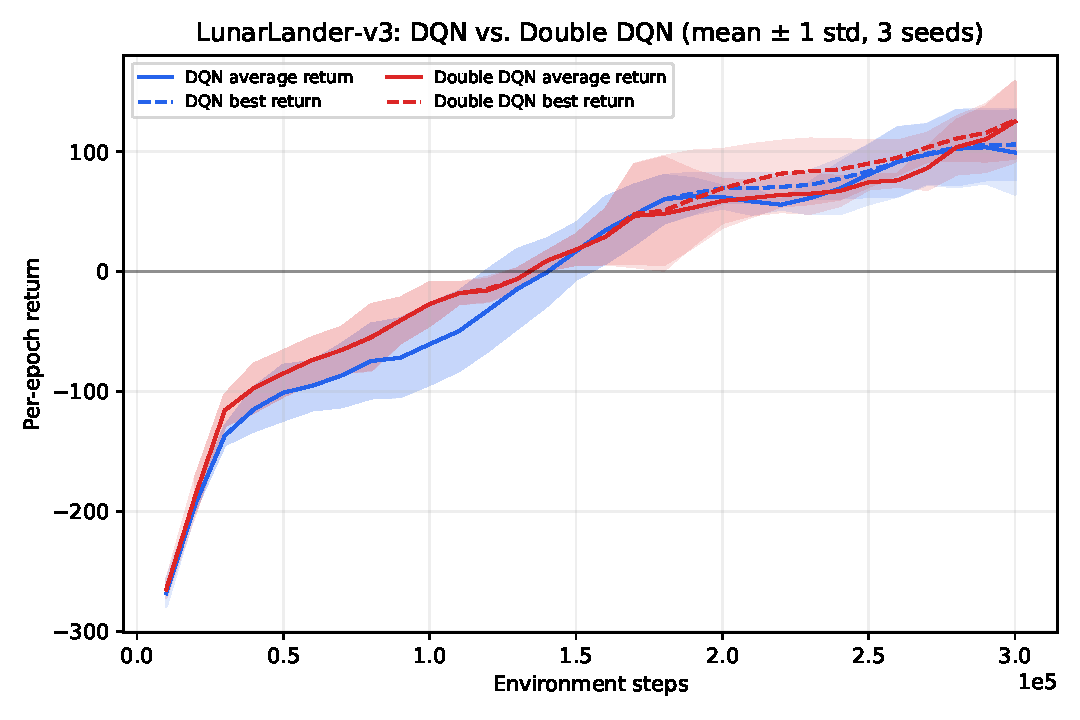
\includegraphics[height=7.4cm,width=\linewidth,keepaspectratio]{figures/q1_dqn_ddqn.pdf}
\par\smallskip
\footnotesize Mean performance across seeds 1--3; shading shows one standard deviation.
Both methods use $\gamma=0.99$, target updates every 2,000 steps, and epsilon
decay from 1.0 to 0.02 over the first 90,000 steps.
\end{answer}

\section{Question 2: Actor-Critic (CartPole-v0) - [3.75 points]}
\begin{answer}[title=Question 2,height=9.5cm,width=\linewidth]
\centering
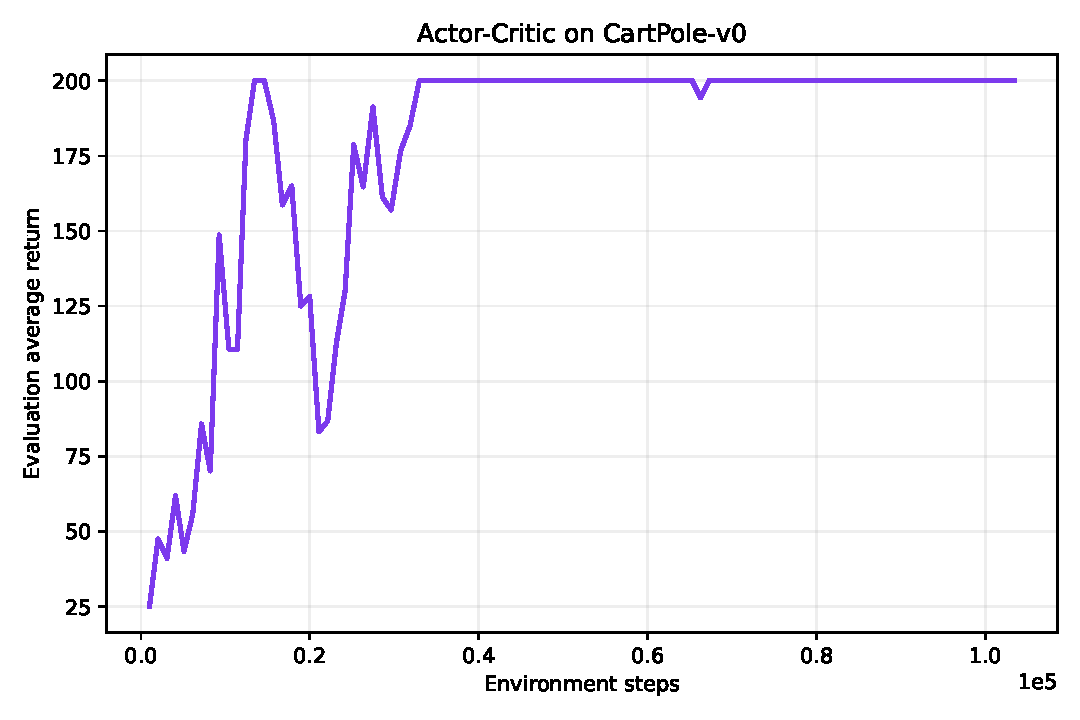
\includegraphics[height=7.6cm,width=\linewidth,keepaspectratio]{figures/q2_cartpole.pdf}
\par\smallskip
\footnotesize Actor-critic reaches the CartPole-v0 maximum return of 200.
\end{answer}



\section{Question 3: Actor-Critic (InvertedPendulum-v4) - [3.75 points]}
\begin{answer}[title=Question 3,height=9.5cm,width=\linewidth]
\centering
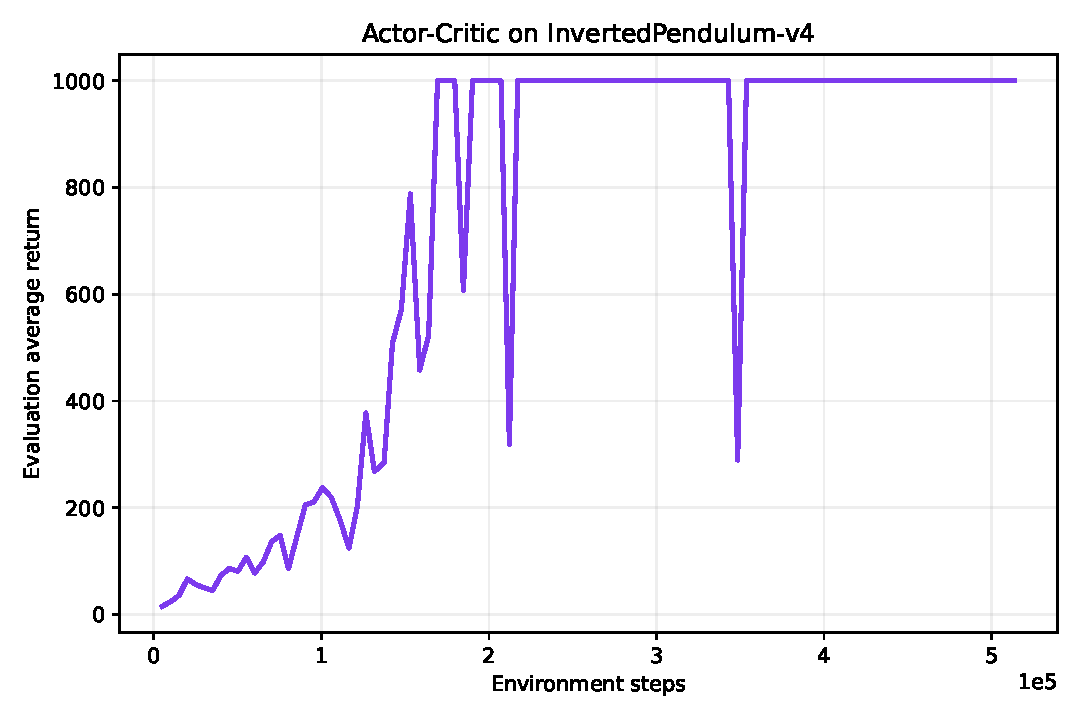
\includegraphics[height=7.6cm,width=\linewidth,keepaspectratio]{figures/q3_inverted_pendulum.pdf}
\par\smallskip
\footnotesize Evaluation return for actor-critic with 10 target updates and 10 gradient steps per target.
\end{answer}







\end{document}
